\section{Language Modelling}\label{sec:lm}

Let a tokenised sequence of length~$T$ be
$\mathbf{x}=(x_{1},x_{2},\dots,x_{T})$.
Under the autoregressive factorisation the joint probability is
\begin{equation}
  P(\mathbf{x})
  \;=\;
  \prod_{t=1}^{T}
  P\!\bigl(x_{t}\mid x_{1{:}t-1}\bigr),
  \label{eq:lm}
\end{equation}
which is maximised during training.
At inference time the model generates tokens sequentially via
\begin{equation}
  x_{t}\sim
  P\!\bigl(x_{t}\mid x_{1{:}t-1}\bigr),
  \qquad
  1\le t\le T,
  \label{eq:lm_next}
\end{equation}
until an end-of-sequence symbol is produced.

\subsection{Transformer Architecture Overview}\label{sec:trf_overview}

The Transformer eliminates the recurrence, and instead we can process all words (i.e tokens) in the sentence at the same time.
both including a self-attention sub-layer followed by a pointwise,
feed-forward network.
Residual connections encompass both of the sub-layers, and the residual branch is, for public release.
immediately normalized.
In the original design layer normalization (LN) was used, however many of the
modern LLMs would prefer the root-mean-squared!
normalizing (RMSNorm) to save computation with no sacrifice of generalization performance.
observable degradation.
Figure~\ref{fig:self_attention} (reproduced) depicts the information
flow through a single self-attention block.
\begin{figure}[h]
    \centering
    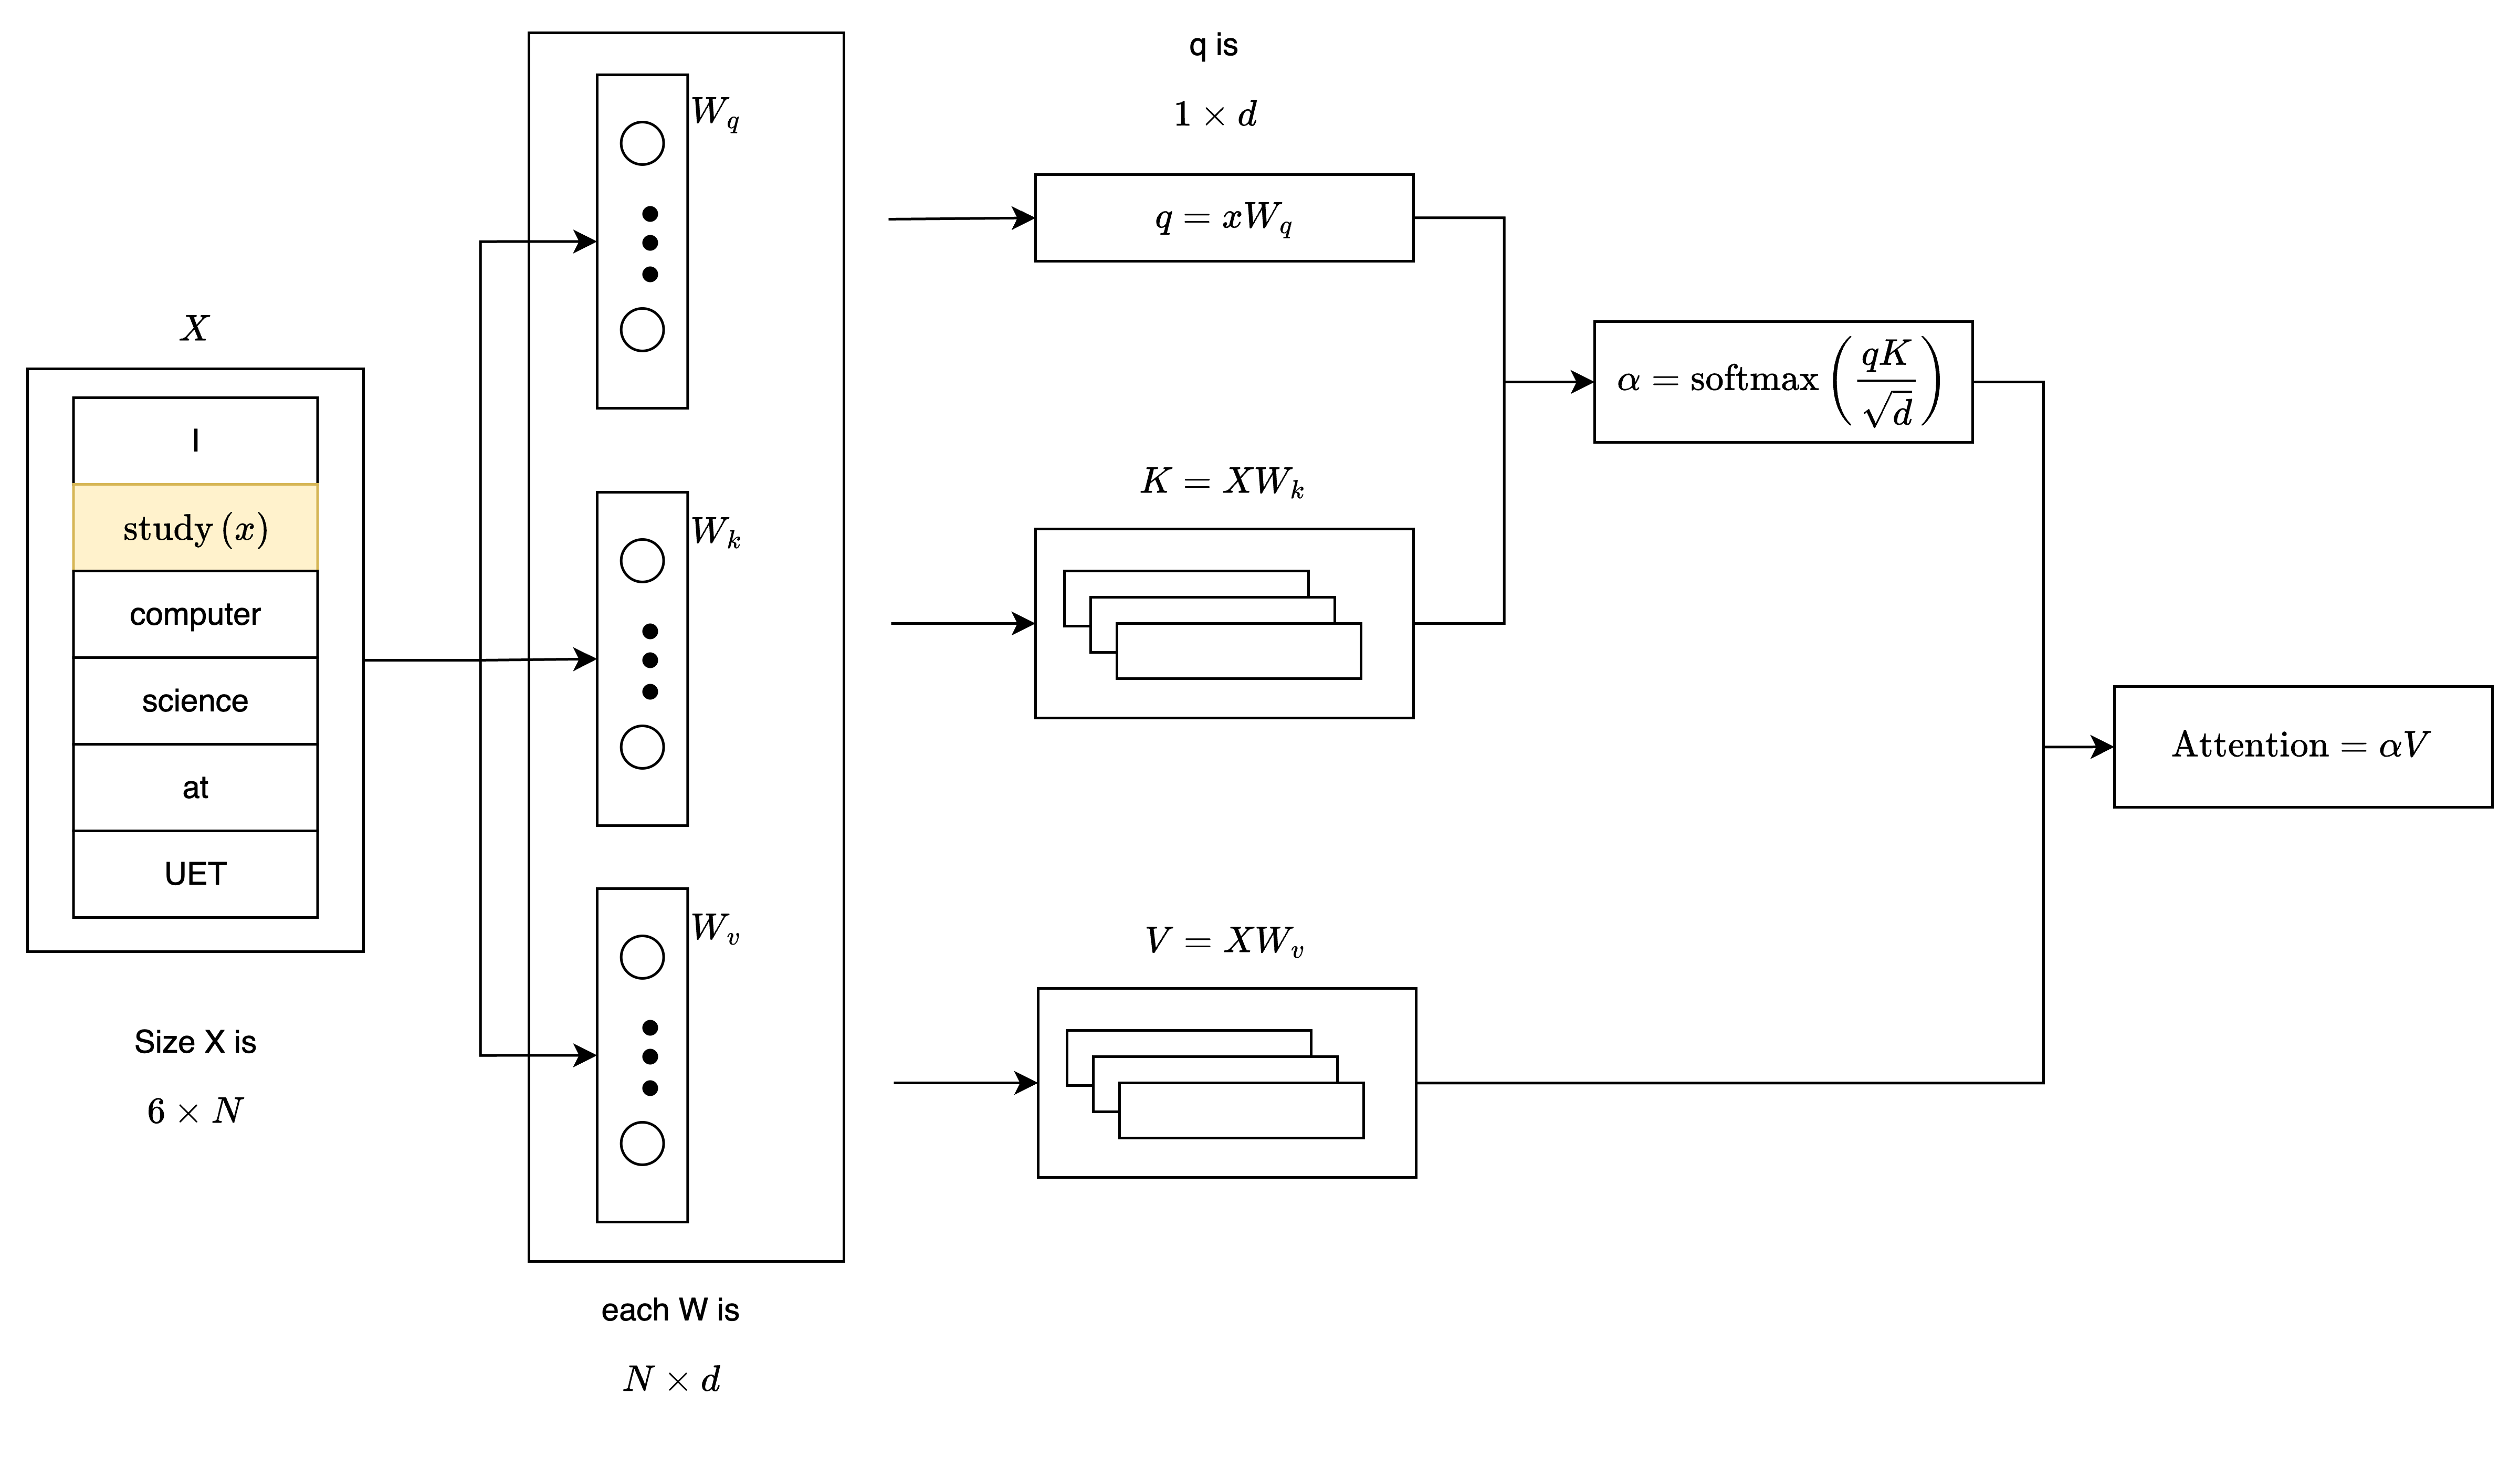
\includegraphics[width=1\linewidth]{figures/c2/self_attention.png}
    \caption{Self-Attention}
    \label{fig:self_attention}
\end{figure}
\subsection{Scaled Dot-Product Self Attention}\label{sec:self_attn}

Given query, key, and value matrices
$\mathbf{Q},\mathbf{K},\mathbf{V}\in\mathbb{R}^{T\times d_{k}}$,
self-attention forms context vectors as
\begin{equation}
  \mathrm{Attn}(\mathbf{Q},\mathbf{K},\mathbf{V})
  \;=\;
  \operatorname{softmax}
  \bigl(
    \mathbf{Q}\mathbf{K}^{\mathsf{T}}/\sqrt{d_{k}}
  \bigr)\mathbf{V},
  \label{eq:attention}
\end{equation}
where the $1/\sqrt{d_{k}}$ factor mitigates gradient vanishing at large
scales.
Multi-head attention replicates~\eqref{eq:attention} $H$ times in
parallel and concatenates the results to enhance representational
capacity.

\subsection{Positional Encodings}\label{sec:pos_enc}

Because the computation in~\eqref{eq:attention} is
permutation-invariant, positional information is injected additively
into token embeddings.
The canonical sinusoidal scheme uses orthogonal sine–cosine waves of
different frequencies, enabling the model to extrapolate to unseen
sequence lengths.  
Recent work replaces absolute sinusoids with \emph{rotary}
positional encodings, which rotate query and key vectors in complex
space and yield superior long-context generalization while keeping the
attention formulation unchanged.

\subsection{Position-Wise Feed-Forward Network}\label{sec:ffn}

Each layer concludes with a two-layer feed-forward network that is
applied identically and independently at every position:
\[
  \mathrm{FFN}(\mathbf{h})
  \;=\;
  \sigma\!\bigl(\mathbf{h}\mathbf{W}_{1}+\mathbf{b}_{1}\bigr)\mathbf{W}_{2}+\mathbf{b}_{2},
\]
where $\sigma$ is typically \textsc{GeLU} or \textsc{SiLU}.
The hidden dimension is usually a multiple (e.g.\ $4\times$) of the
model dimension, providing a widening–compression pattern that
increases expressiveness with modest parameter cost.

\subsection{Normalization and Residual Pathways}\label{sec:norm_res}

Residual connections allow gradients to propagate directly through the
network depth, facilitating optimisation of very deep stacks.
Layer norm standardises activations per hidden unit, whereas RMSNorm
scales only by the root-mean-square of each vector, marginally
reducing computation and improving numerical stability in low-precision
training.
Both normalizations are applied \emph{pre-activation} in many modern
LLMs, a change that eases training dynamics compared to the original
post-activation formulation.

\subsection{Inference-Time Optimizations}\label{sec:kv_cache}

During autoregressive generation the model repeatedly attends to the
entire prefix $\mathbf{x}_{1{:}t-1}$.
Caching key–value tensors for previously generated tokens eliminates
quadratic recomputation, shrinking complexity per step from
$\mathcal{O}(t^{2})$ to $\mathcal{O}(t)$.
Further memory reductions can be obtained with structured compression
(e.g.\ product-quantised or low-rank caches) that store keys and values
in compact form and decompress them on the fly.

\subsection{Grouped-Query Attention}\label{sec:gqa}

In standard multi-head attention each head owns distinct projections
for queries, keys, and values.
Multi-query attention shares one key–value pair across all heads,
considerably decreasing memory and latency.
Grouped-query attention situates itself between these extremes by
partitioning the $H$ query heads into $G$ disjoint groups that share
key–value projections within—but not across—groups.
The special cases $G=H$ and $G=1$ recover MHA and MQA, respectively.

\subsection{Scaling and Training Considerations}\label{sec:scaling}

Empirical scaling laws reveal that pre-training loss decays as a
power-law in model size, data, and compute, suggesting predictable
returns on investment in larger models.
To train beyond single-GPU memory limits modern stacks rely on AdamW
optimisation, mixed-precision arithmetic, gradient-checkpointing, and
ZeRO-style parameter/state sharding.
These techniques jointly amortise compute and memory costs, enabling
hundreds-of-billion-parameter models to converge within practical
budgets.
